\begin{center}
	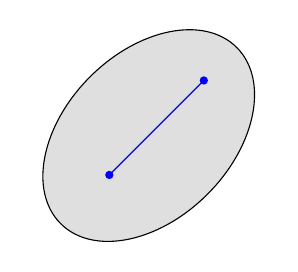
\begin{tikzpicture}
	\draw[rotate=-45,fill=gray!25] (0,0) ellipse (30pt and 45pt);
	\textcolor{blue}{
		\draw (-0.5,-0.5) -- (0.7,0.7);
		\fill (-0.5,-0.5) circle[radius=1.5pt];
		\fill (0.7,0.7) circle[radius=1.5pt];
	}
	%\draw (-0.7,0.6) node[below] {\Large $C$};
	\end{tikzpicture}
	\qquad \qquad
	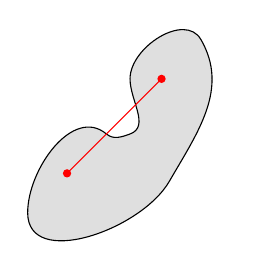
\begin{tikzpicture}
	\useasboundingbox (-1,-1.35) rectangle (1.5,1.35);
	\draw[fill=gray!25] (0,0) to [out=140,in=90] (-1,-1)
	to [out=-90,in=240] (0.8,-0.6)
	to [out=60,in=-60] (1.2,1.2)
	to [out=120,in=90] (0.3,0.7)
	to [out=-90,in=20] (0.3,0)
	to [out=200,in=-40] (0,0);
	\textcolor{red}{
		\draw (-0.5,-0.5) -- (0.7,0.7);
		\fill (-0.5,-0.5) circle[radius=1.5pt];
		\fill (0.7,0.7) circle[radius=1.5pt];
	}
	%\draw (0.3,-0.2) node[below] {\Large $N$};
	\end{tikzpicture}
	\captionof{figure}{links: konvexe Menge, rechts: keine konvexe Menge}
\end{center}